\section{Evaluation}\label{sec:evaluation}
We have already looked at other results in the literature in section \ref{sec:practical-results-lit} which gave a decent comparison between some of the algorithms. However, we did not get a lot of knowledge about the datasets, especially the structure of the preference list and distribution of those preferences. Therefore we will conduct an experiment, by benchmarking the implemented algorithms with both real and artificial datasets of varying sizes and preference structures.

\subsection{Research Questions}
Table \ref{tab:algorithm-comparison} already compared and summarized the algorithms from a theoretical perspective, however some of the results would benefit from further quantification and clarity. For instance, we know that the Max-Popular algorithm, as described in section \ref{algo-max-pop}, does not always produce a matching. It would be beneficial to empirically investigate if certain inputs cause this problem. Therefore we will formalize some open questions as research questions, that this experiment hopes to answer:
\begin{enumerate}
    \item What is the effect of different preference distributions on the matchings produced by the different algorithms.
    \item How likely is it for the Max-Popular algorithm to not produce a matching using different datasets?
    \item How does the Modified-Popular algorithm from section \ref{impl:mod-max-pop} compare in terms of popularity to the other algorithms.
    \item What is the cost of giving up on strategy proofness in terms of rank, i.e. how well does RSD perform compared to other mechanisms?
    \item Is Popularity a meaningful metric for the student-seminar use case?
    \item What is the impact of short-preference lists on the quality and existence of matchings?
\end{enumerate}

\subsection{Sample Data}
Due to the fact that real data for seminar registrations is mostly kept private, a majority of the benchmark will rely on synthetic data. However, there are a few publicly available datasets available that will be used for evaluation and also for better understanding real-world preference distributions.

\subsubsection{Using graph generators}
Using graph generators to synthetically create instances to the seminar-student matching problem turned out to be a big challenge. Essentially, we would need a graph generator for bipartite, weighted graphs, that also considers the seminar capacity. One option would be generating as many nodes as the total capacity of all seminars, but that could result in duplicate edges or i.e. preferences. Therefore we will use a custom, domain specific mechanism for generating instances.

\subsubsection{Random Uniform Preference Lists}
Probably the simplest way to synthetically generate data, was picking a size for the instance and then generating seminars and students based on a uniform random generator. The preference lists are created by shuffling the list of all seminars for each student. Additionally, we can simply shorten each preference list by a random factor as well for measuring the effect of incomplete-preference lists.

\subsubsection{PrefLib Datasets}
Preflib.org is an open collection of more than 3000 community-contributed datasets of preference data for different domains \cite{PrefLib}. Fortunately, there exist two datasets of students' course preferences at the polish AGU University \cite{preflib-dataset}. The two datasets contain strict and complete preference lists for each students with 9 courses and 146 students or 7 courses and 153 students respectively. Unfortunately there are no capacities given, however those will be computed synthetically using a uniform distribution. An interesting characteristic of those dataset is that in each dataset, all students rank the same seminar with their first preference. I decided to those seminars from the dataset, because I wouldn't assume such a preference distribution in the real world.

\begin{figure}[h!]
    \centering
    \begin{subfigure}[b]{0.49\linewidth}
      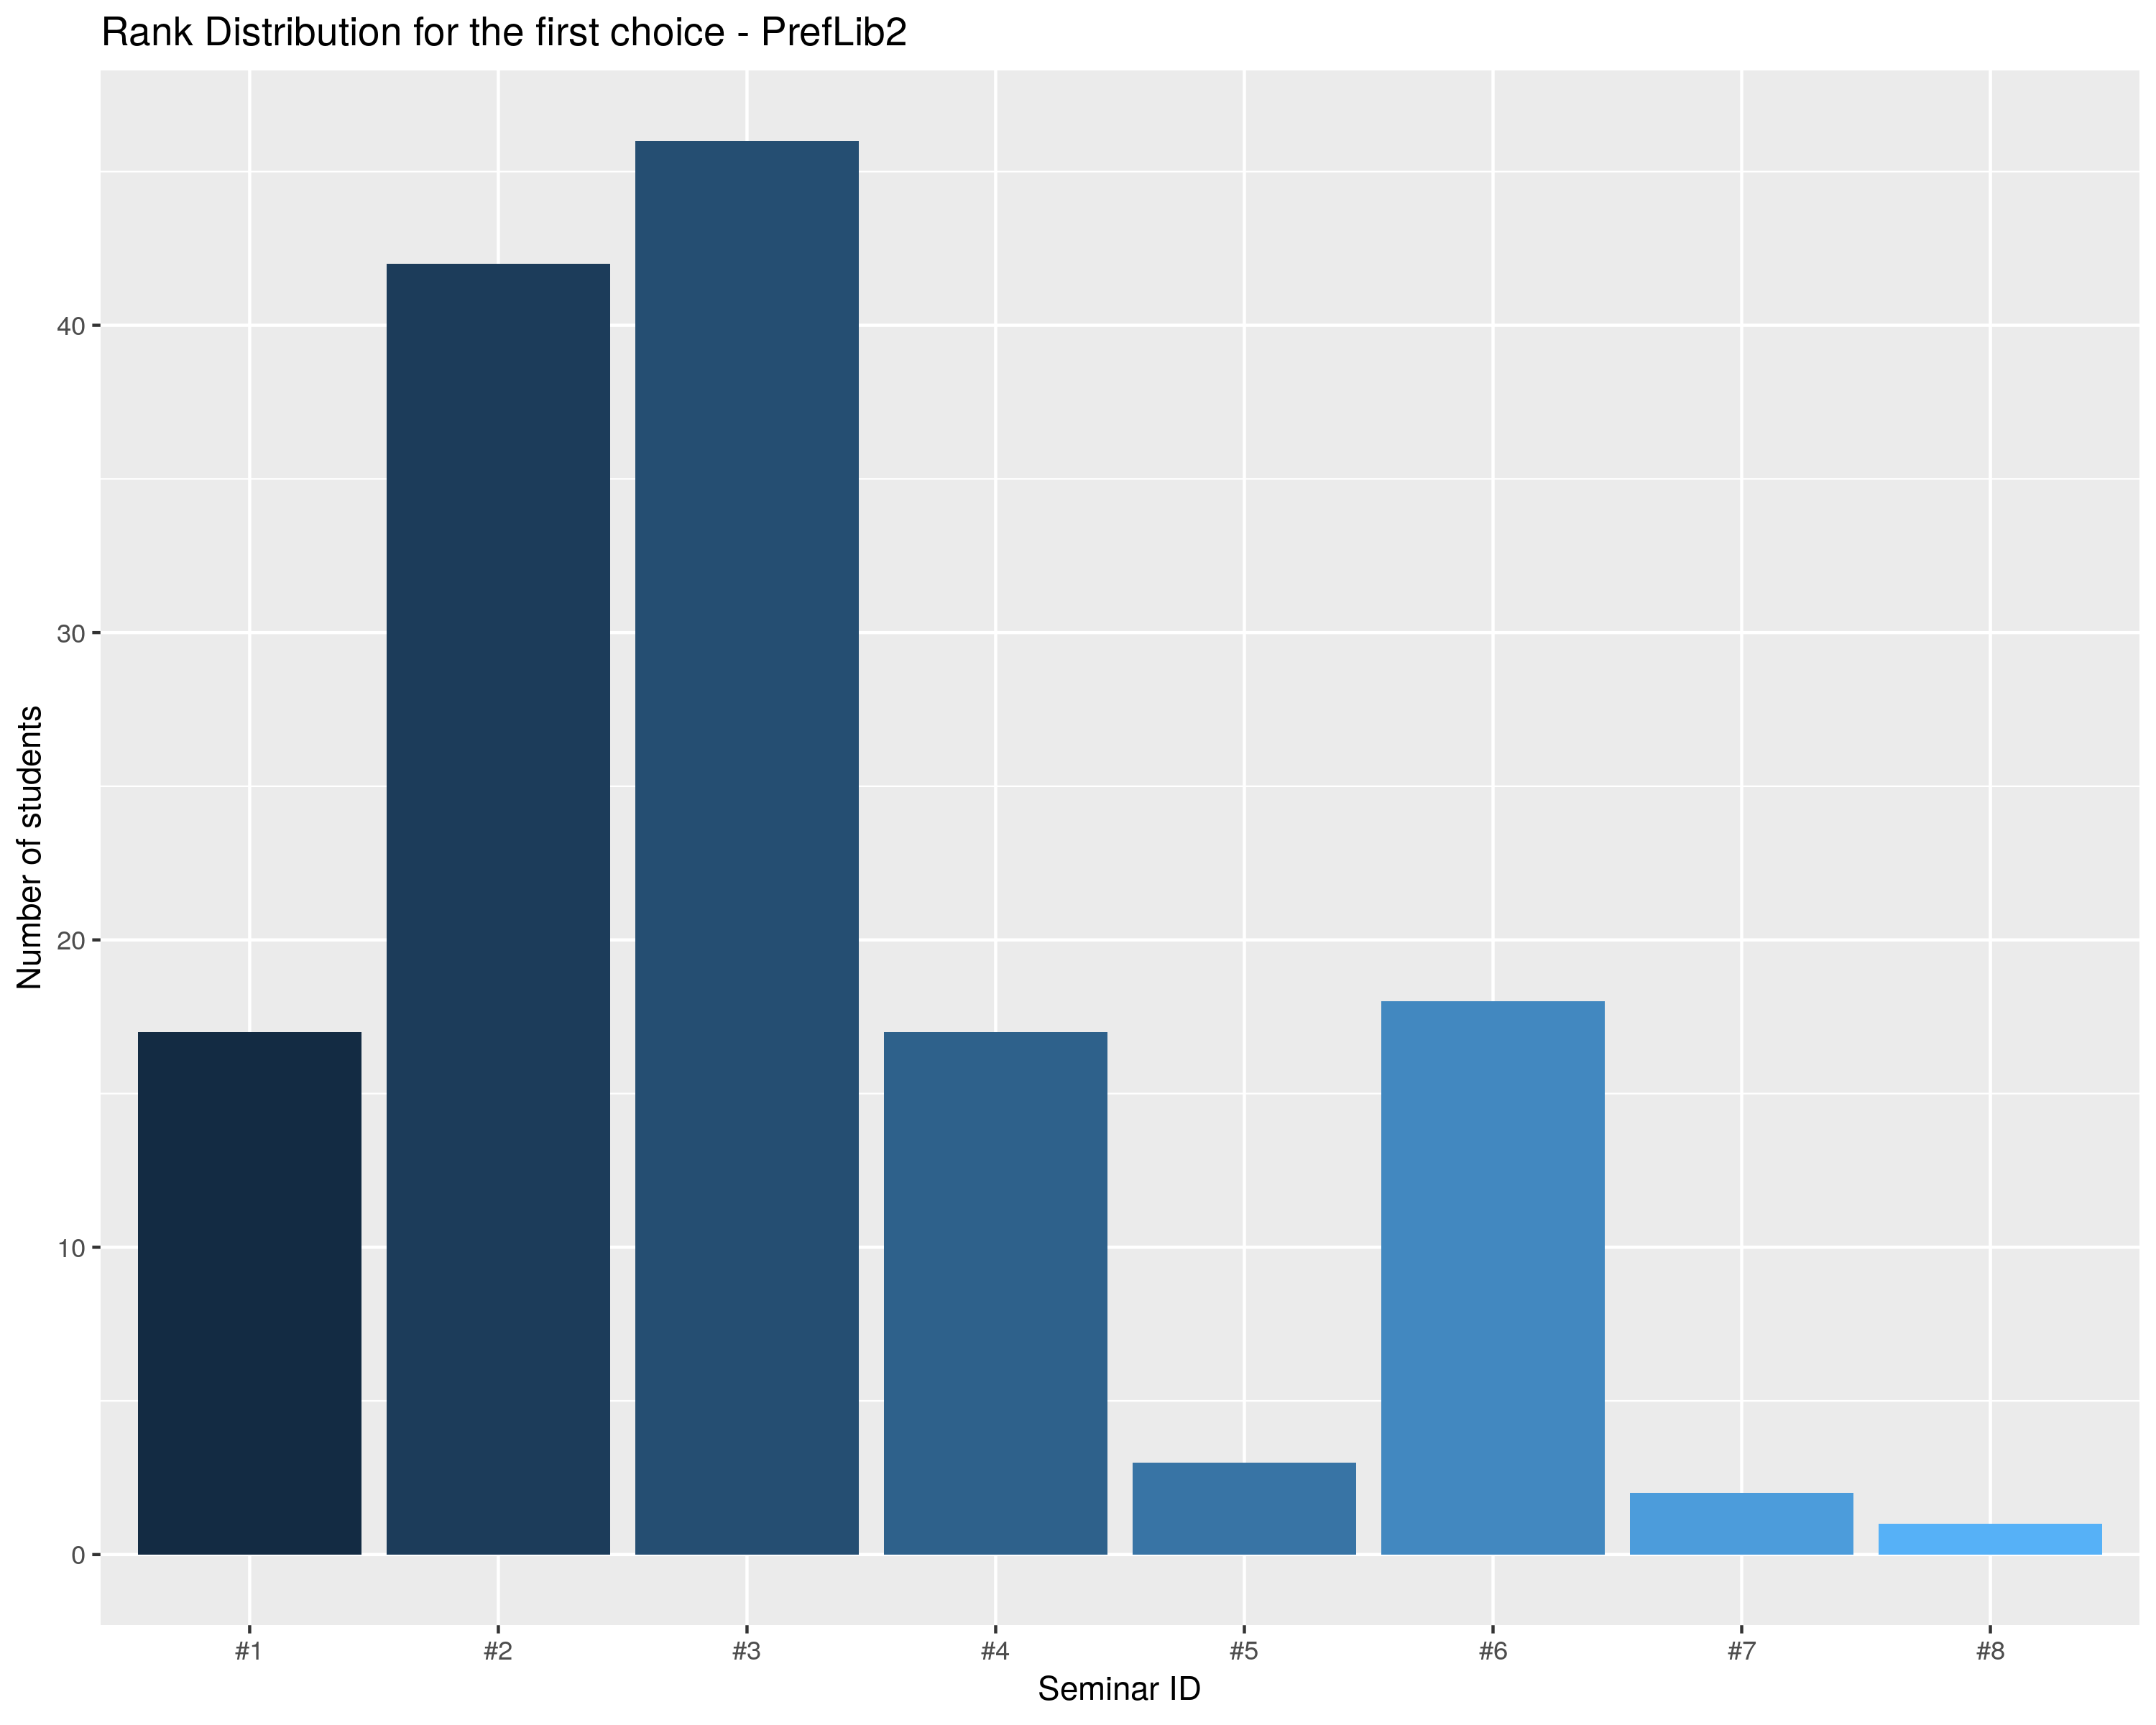
\includegraphics[width=\linewidth]{assets/plots/preflib1-distribution.png}
      \caption{Preference Distribution first dataset.}
    \end{subfigure}
    \begin{subfigure}[b]{0.49\linewidth}
      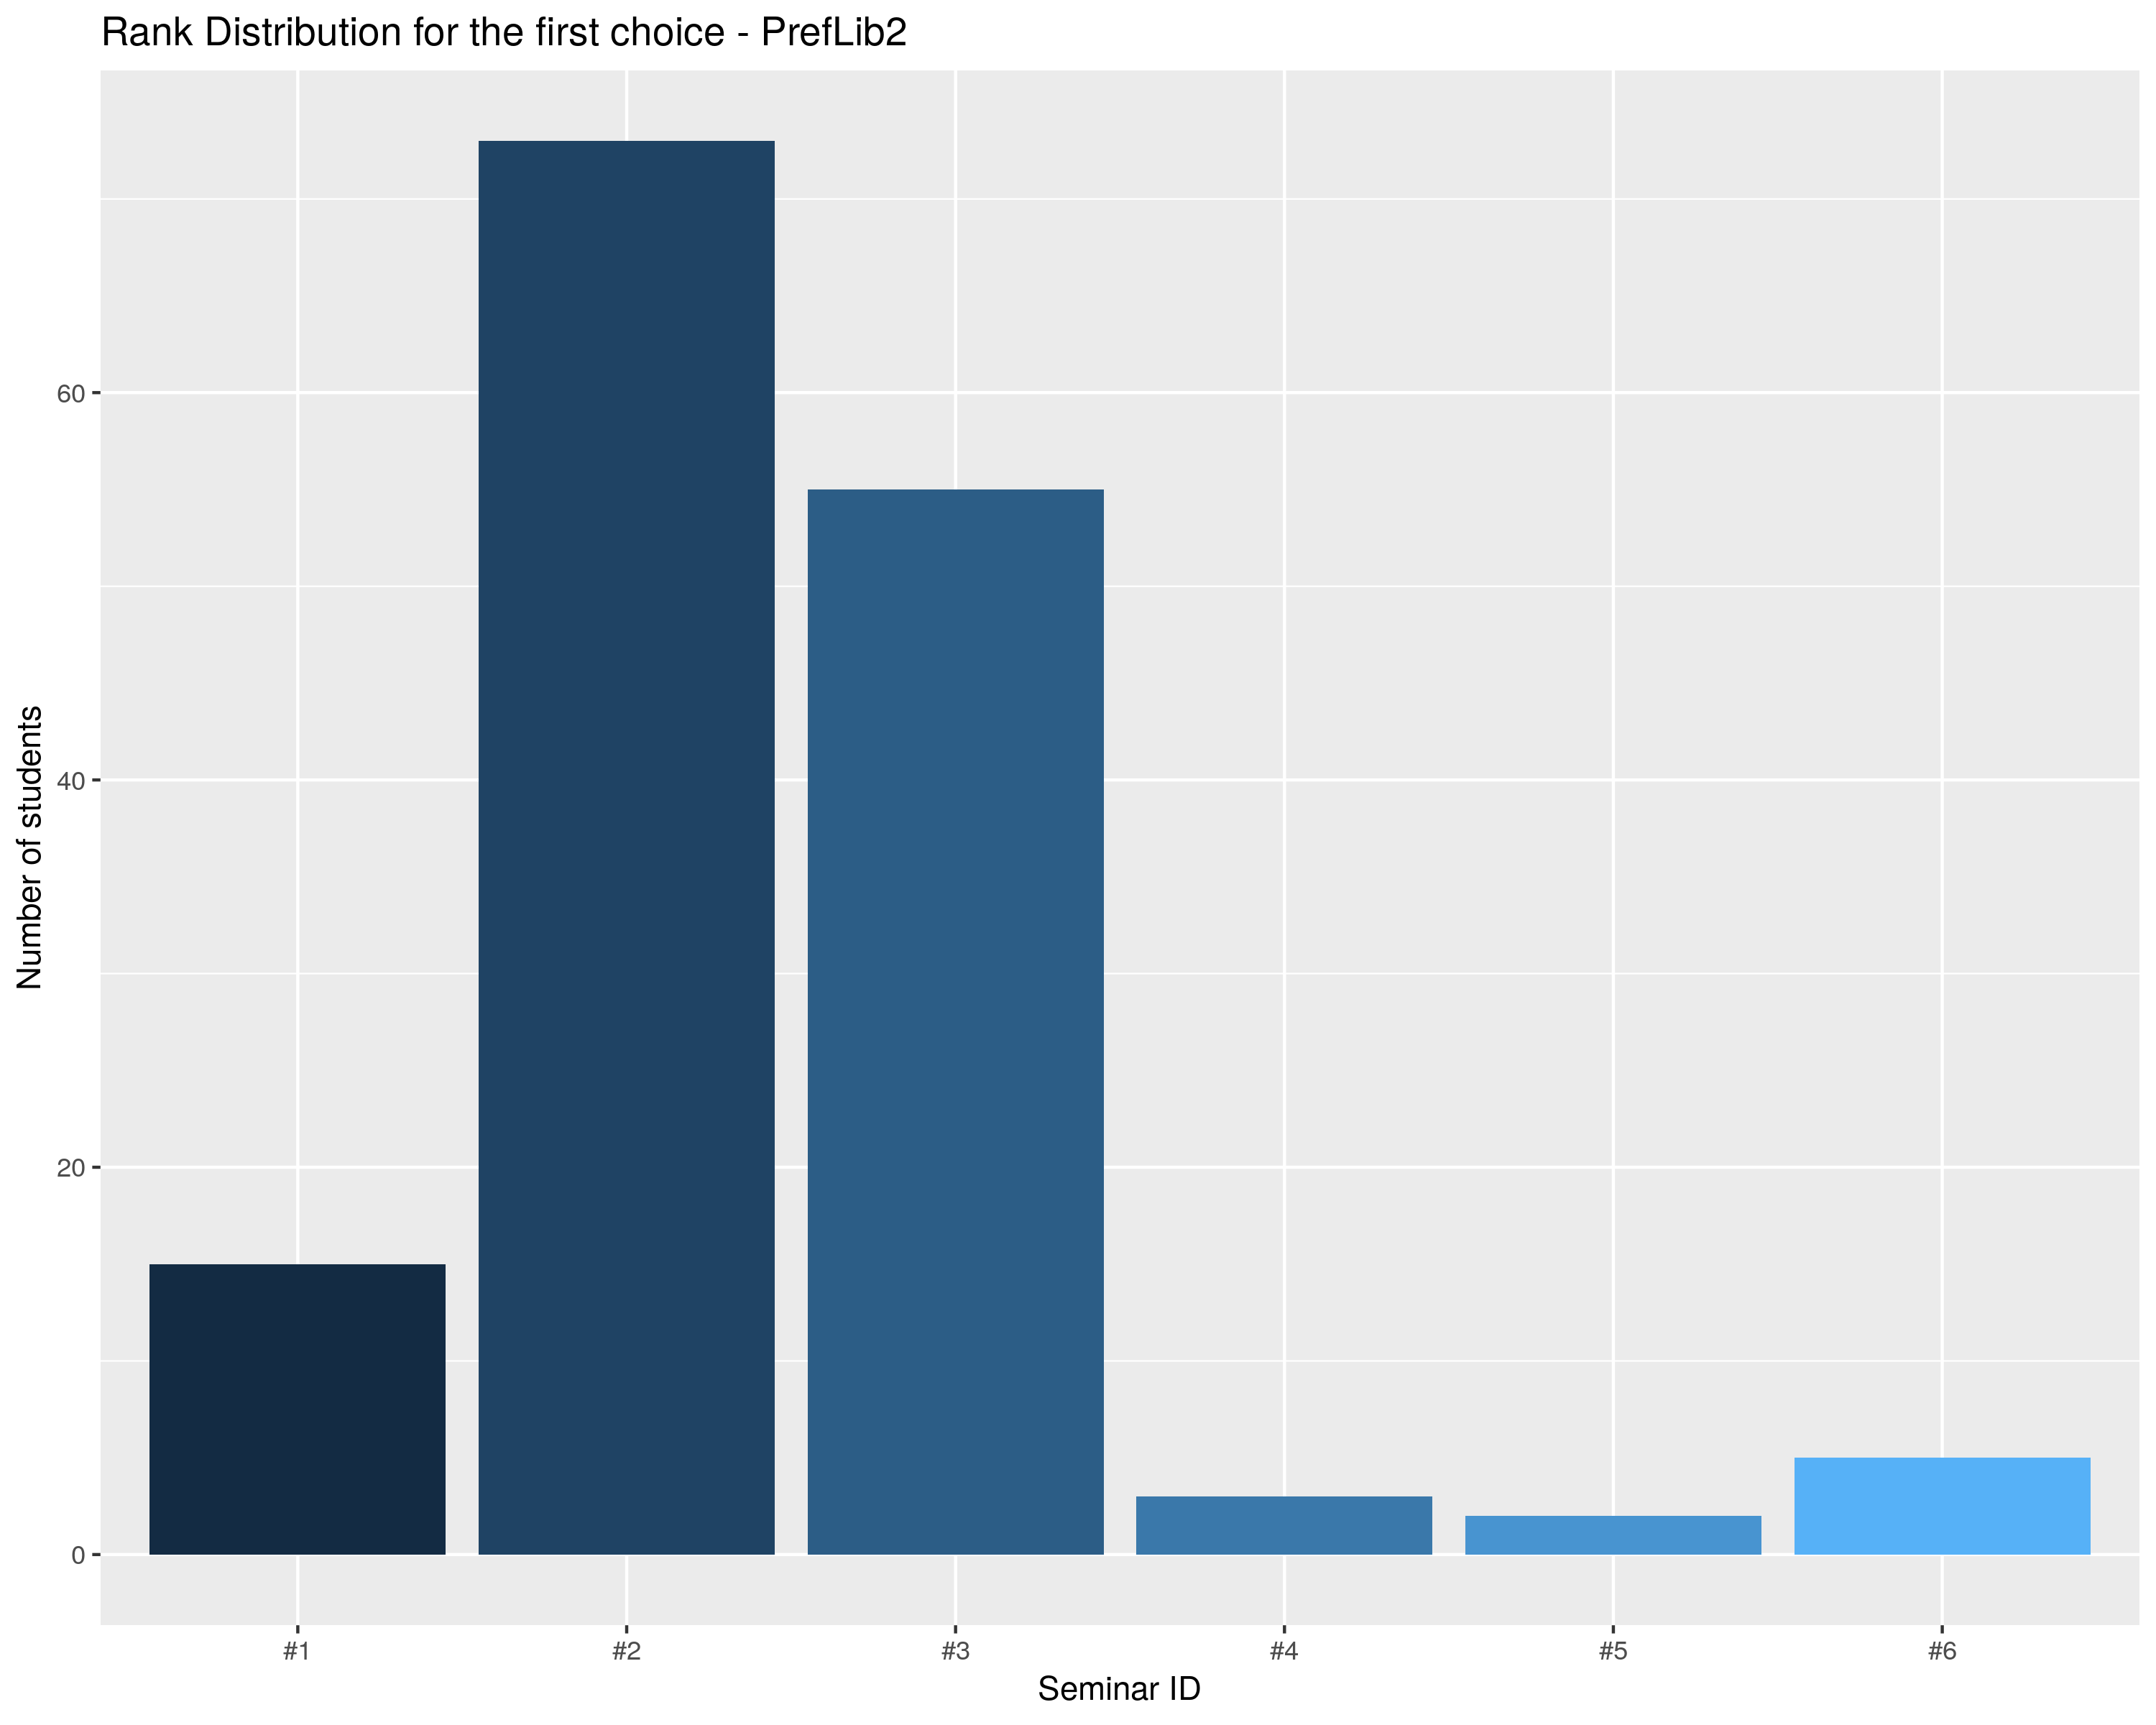
\includegraphics[width=\linewidth]{assets/plots/preflib2-distribution.png}
      \caption{Preference Distribution second dataset.}
    \end{subfigure}
    \caption{Preference Distributions for first-ranked seminars for both PrefLib datasets}
    \label{fig:preflib-distribution}
  \end{figure}

Figure \ref{fig:preflib-distribution} shows the preference distributions for the student's first choice in both datasets after removing the always first-ranked seminar. We can see that in both datasets, students clearly strongly prefer two seminars. However in the first dataset, there are 3 more seminars that are also decently popular, while in the second dataset the majority of students really prefers the two dominant seminars. Generally, those datasets indicate that the preference structure is perhaps not likely to be uniformly distributed.

\subsubsection{Random Zipf-Distributed Preference Lists}
To better simulate real-world preference structures than by using a uniform distribution, a power-law distribution can be applied. According to Zipf's law the frequency of a word in a large sample, is proportional to it's position in a frequency table. This law can also be applied for creating synthetic seminar distribution. Using this type of distribution with some additional randomization yields the following preference list structure when seminar and student counts are similar to the first PrefLib dataset:

\begin{figure}[h!]
    \centering
    \begin{subfigure}[b]{0.49\linewidth}
      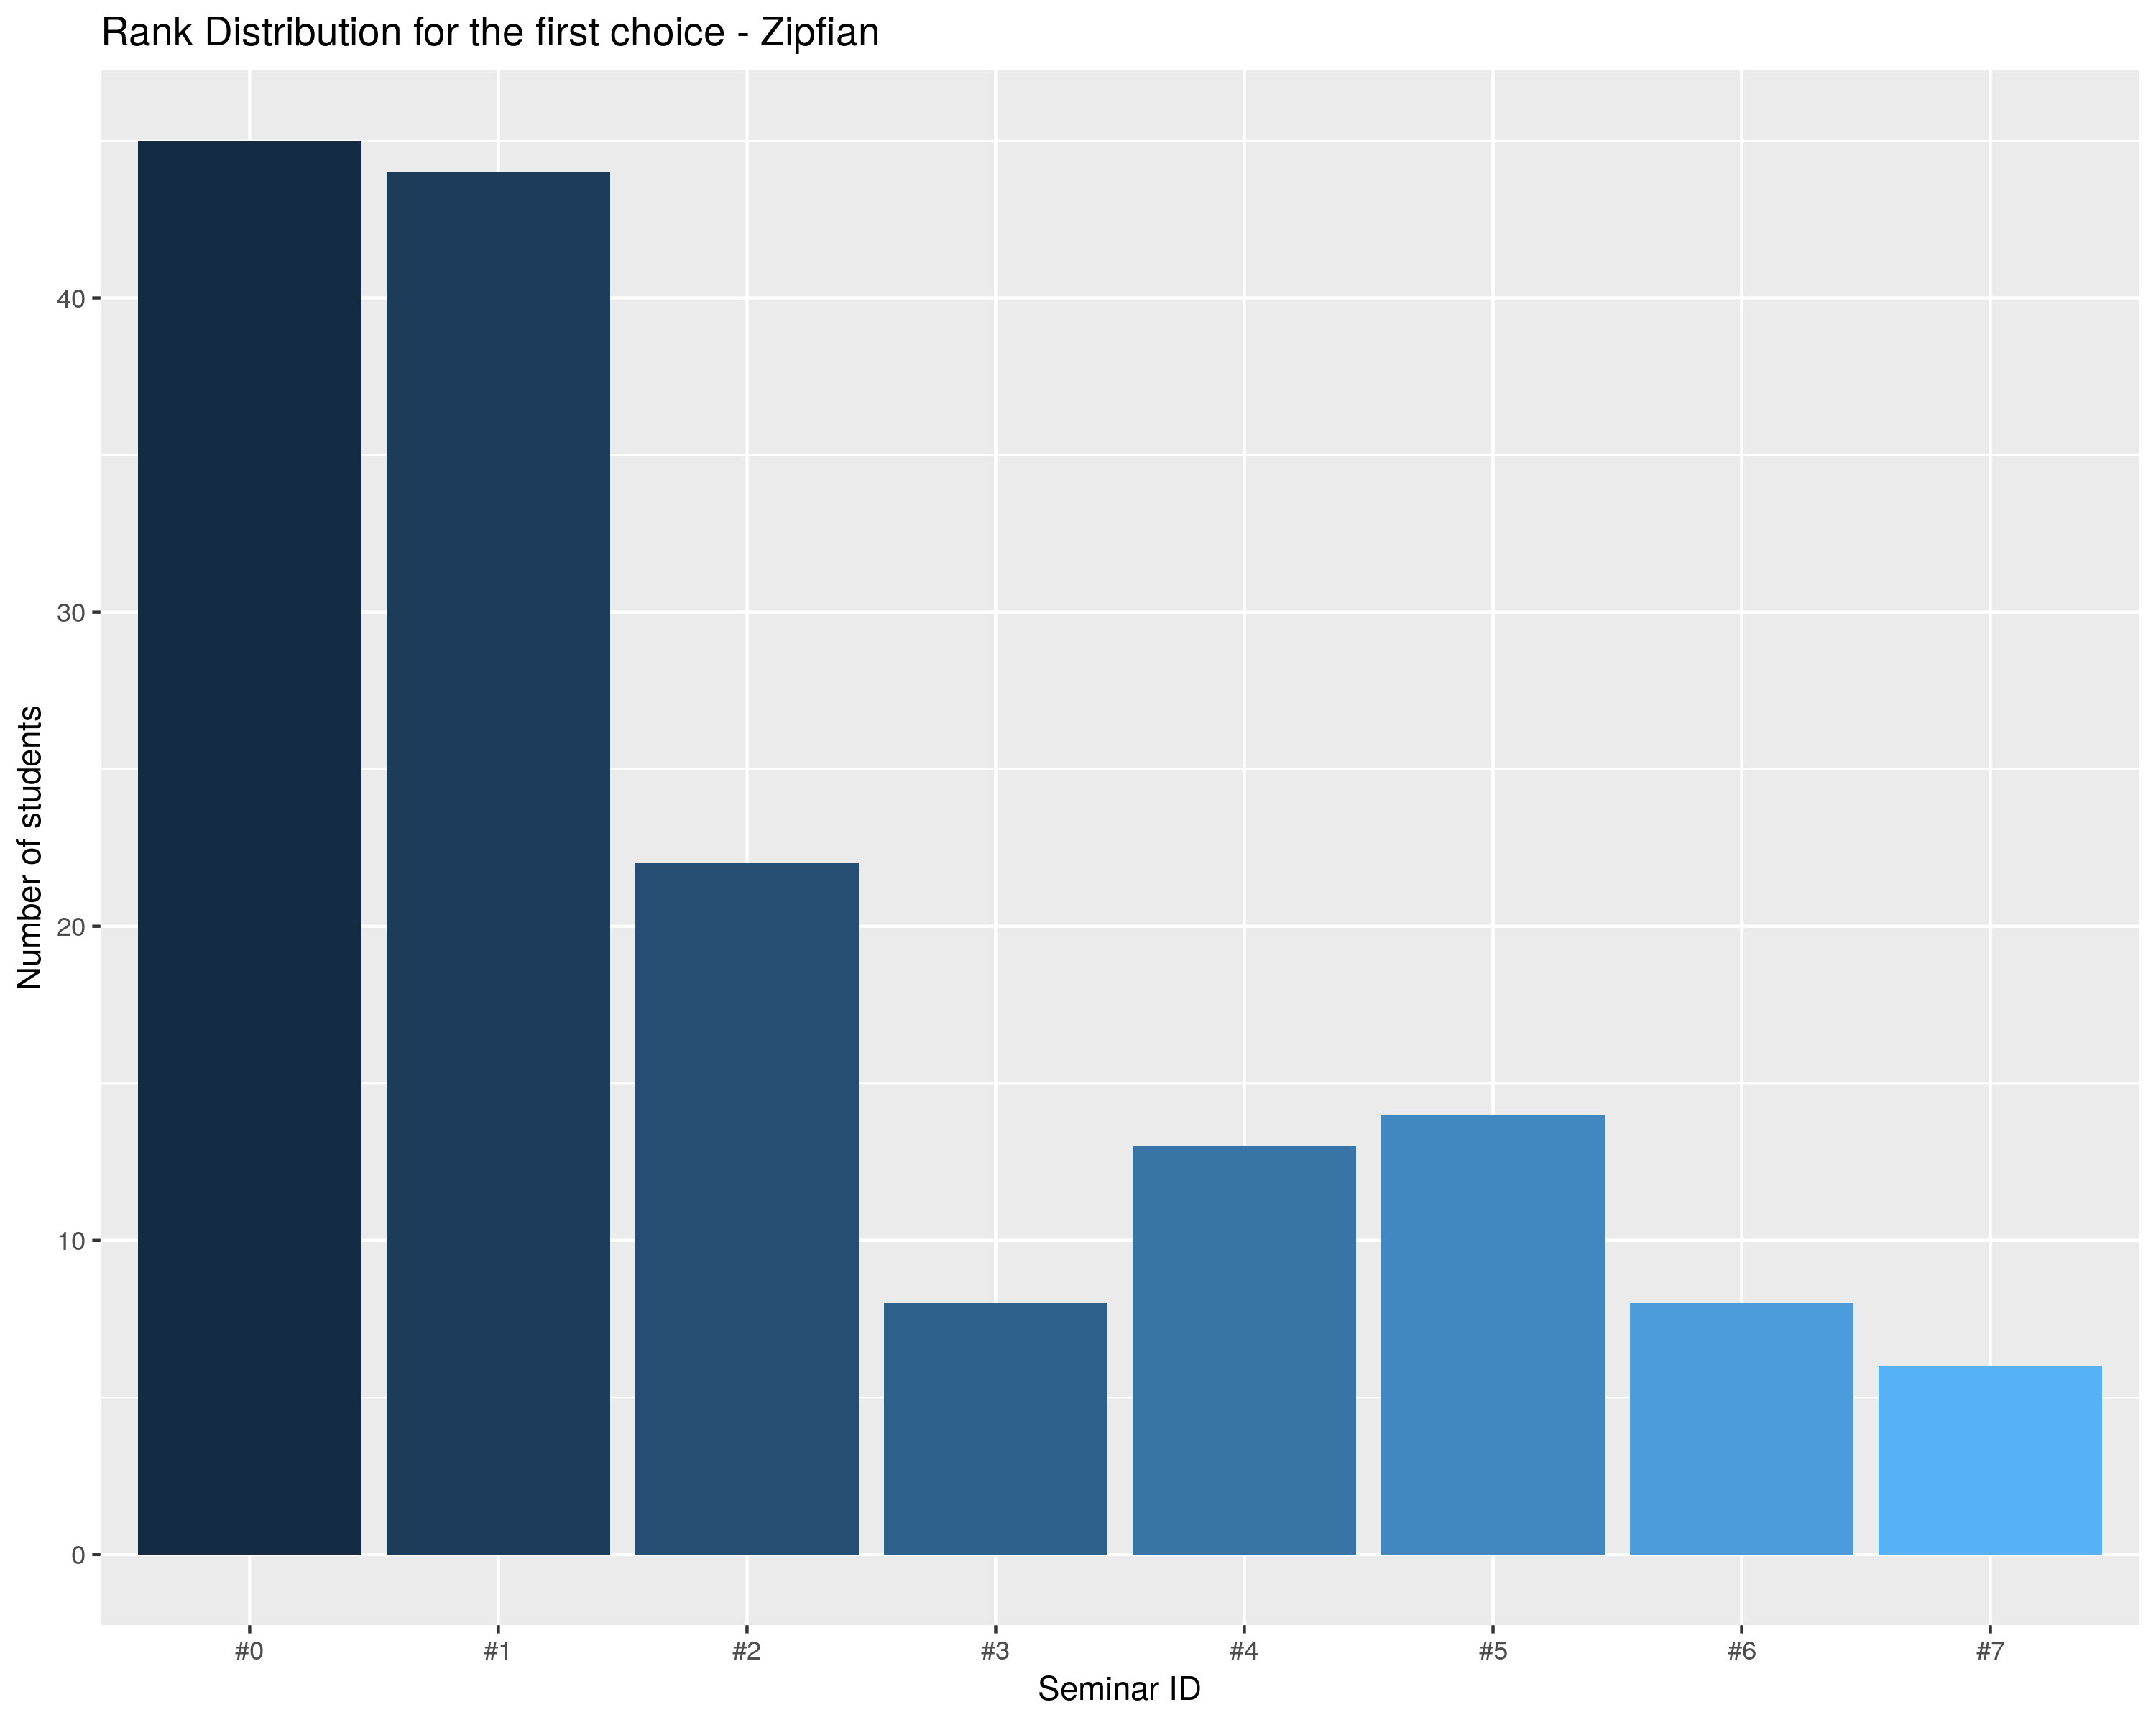
\includegraphics[width=\linewidth]{assets/plots/zipfian1-distribution.png}
      \caption{Preference Distribution first sample.}
    \end{subfigure}
    \begin{subfigure}[b]{0.49\linewidth}
      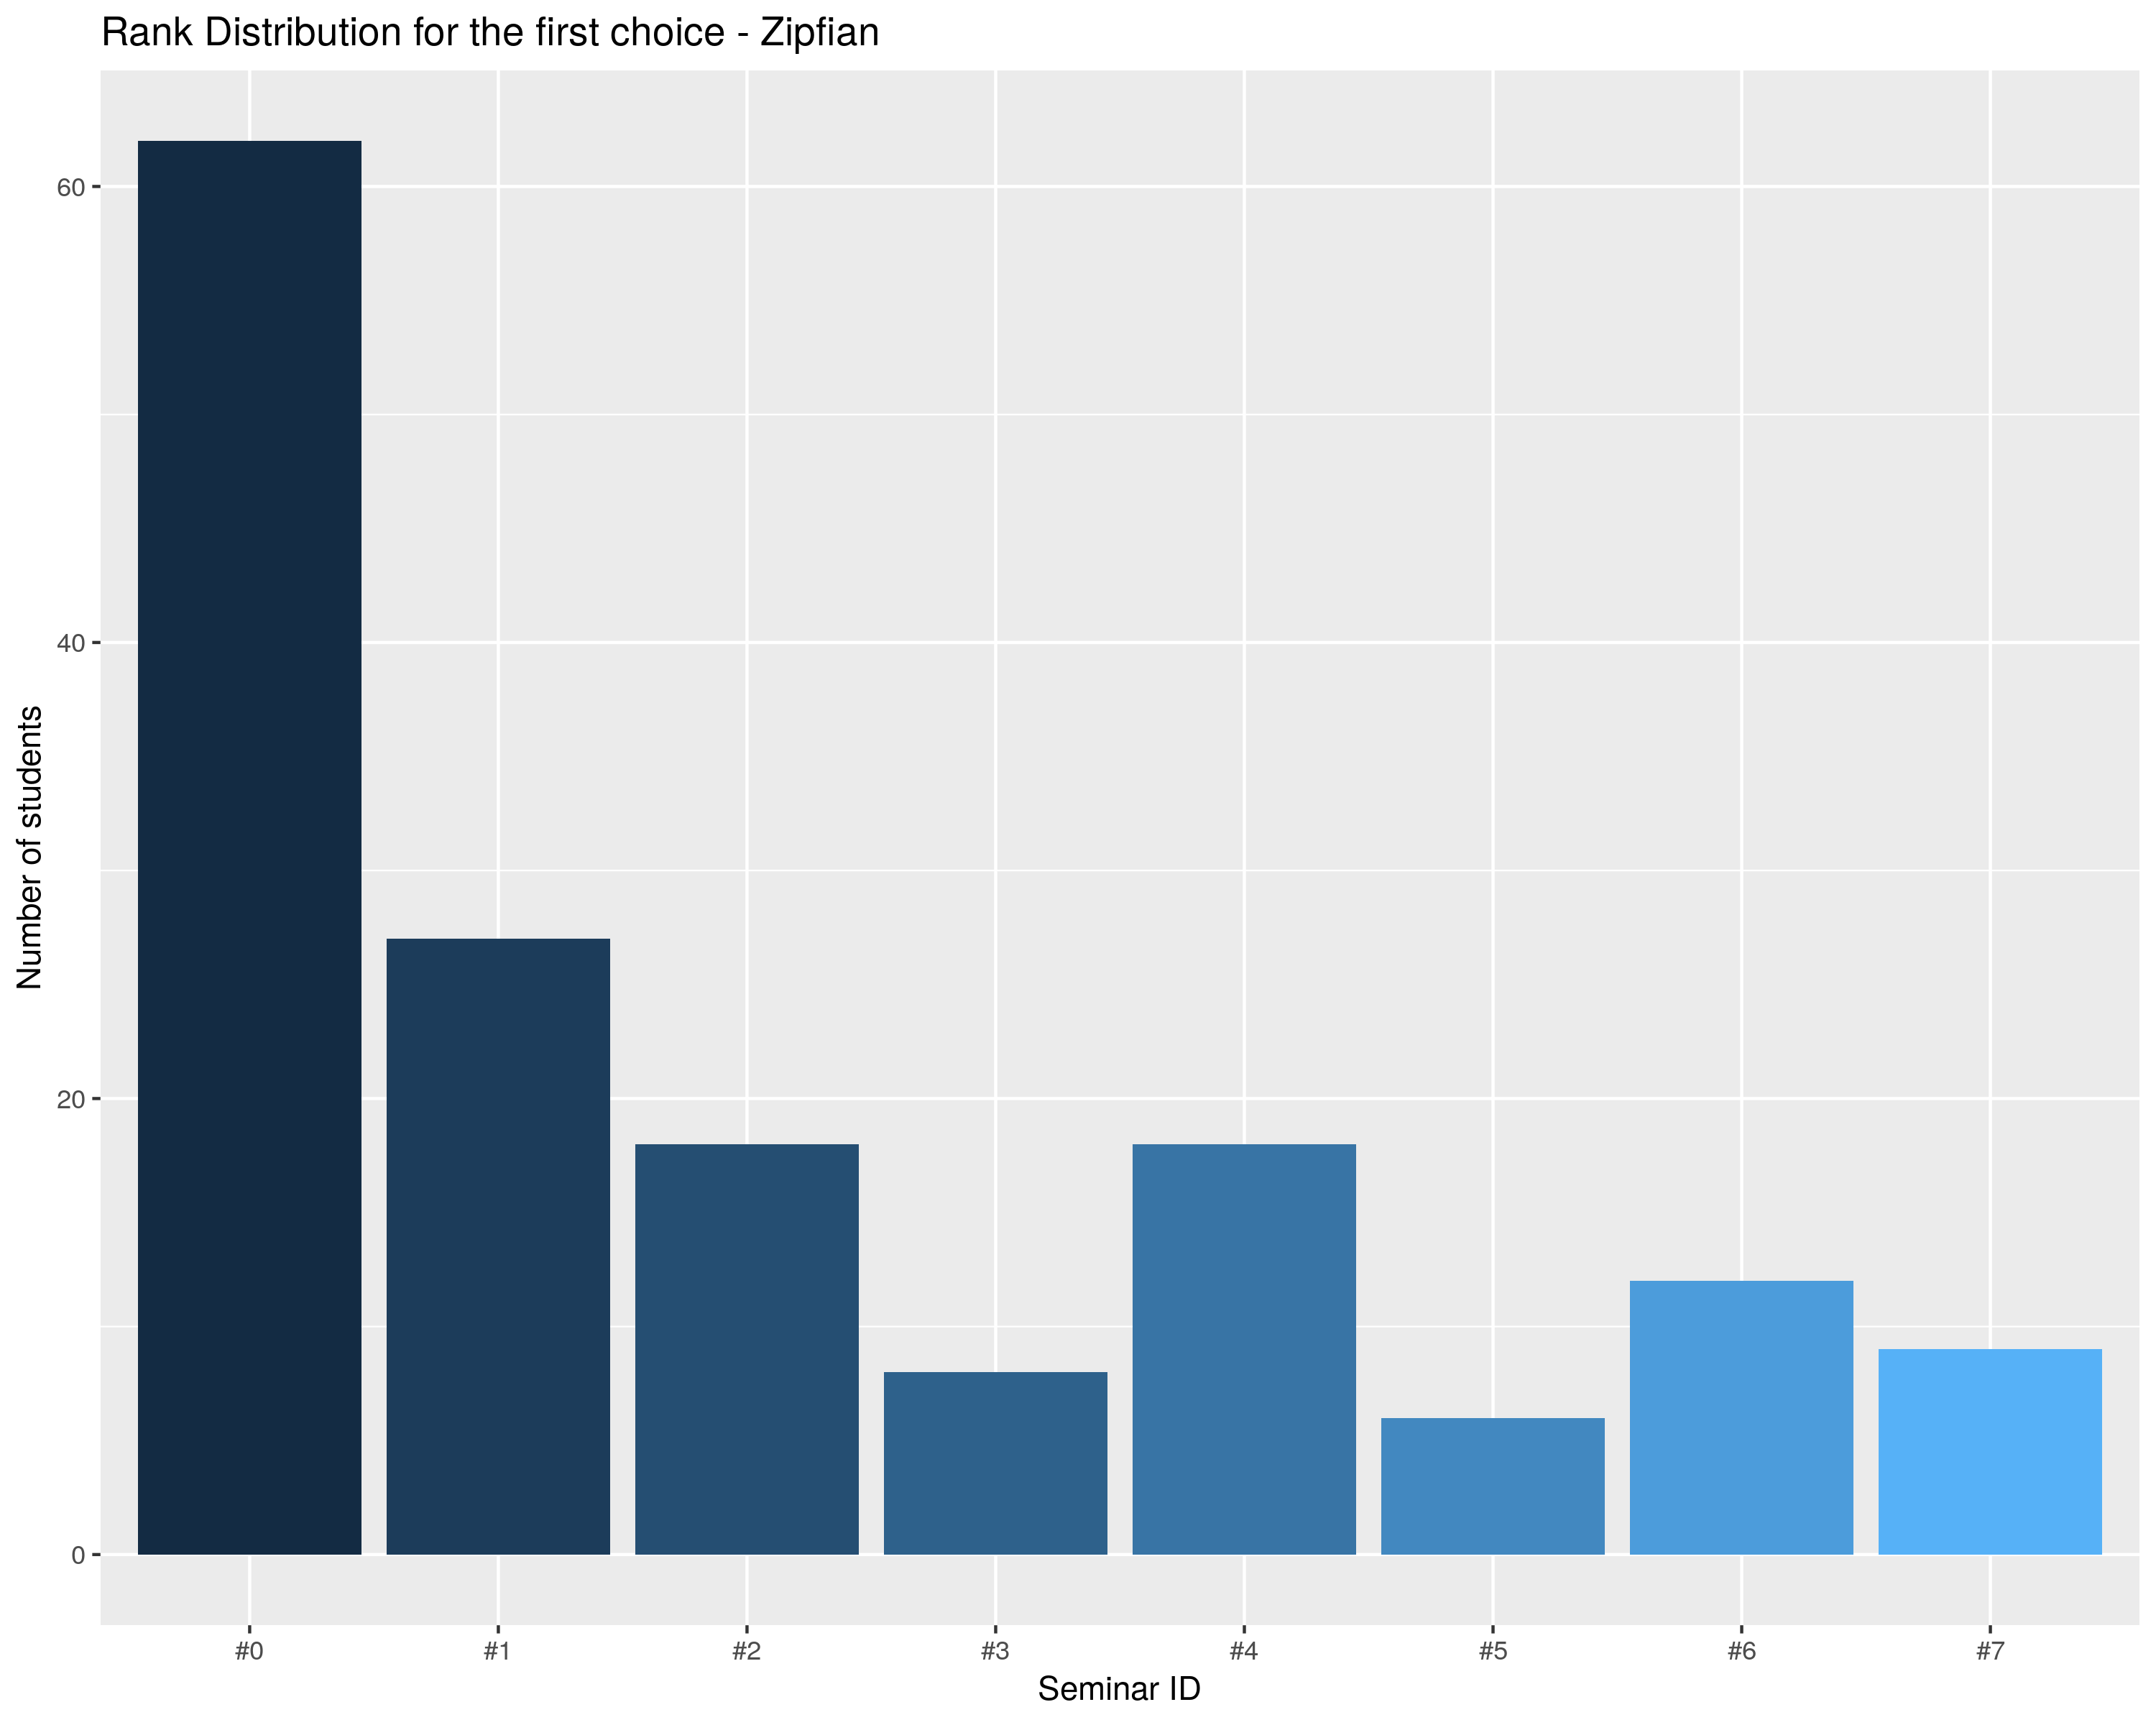
\includegraphics[width=\linewidth]{assets/plots/zipfian2-distribution.png}
      \caption{Preference Distribution second sample.}
    \end{subfigure}
    \caption{Zipfian Preference Distribution for first-ranked seminars}
    \label{fig:zipfian-distribution}
  \end{figure}

To create the dataset, for each student a seminar is randomly drawn using the Zipfian distribution and added to the his preference list until the desired preference-list length has been reached. Comparing Figure \ref{fig:zipfian-distribution} to Figure \ref{fig:preflib-distribution} shows somewhat similar results, which should make this generator relevant for the benchmark. 

\subsubsection{Carnegie-Mellon Datasets}

\subsection{Methodology}
-worst rank
-avg rank /stdeviation
-profile
-cardinality
-popularity
-time

\subsection{Results}

\subsection{Conclusion}